\begin{figure}[H]
    \centering
    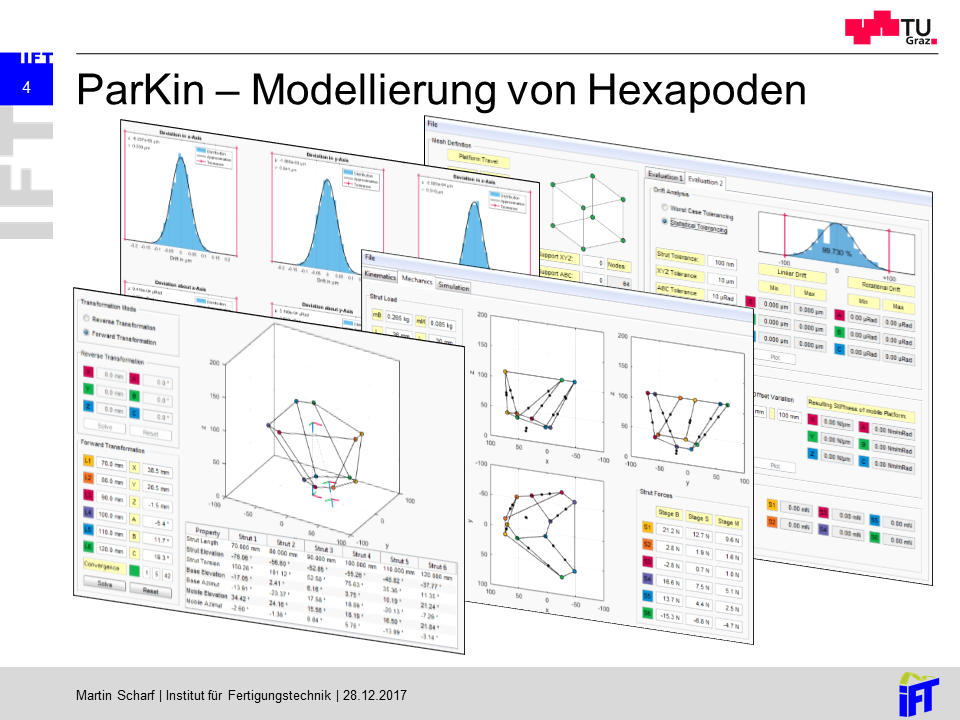
\includegraphics[width=0.7\textwidth]{method/parkin1}
    \caption[Folie]{Folie, Quelle: Eigene Darstellung}
    \label{fig:parkin1}
\end{figure}

\begin{figure}[H]
    \centering
    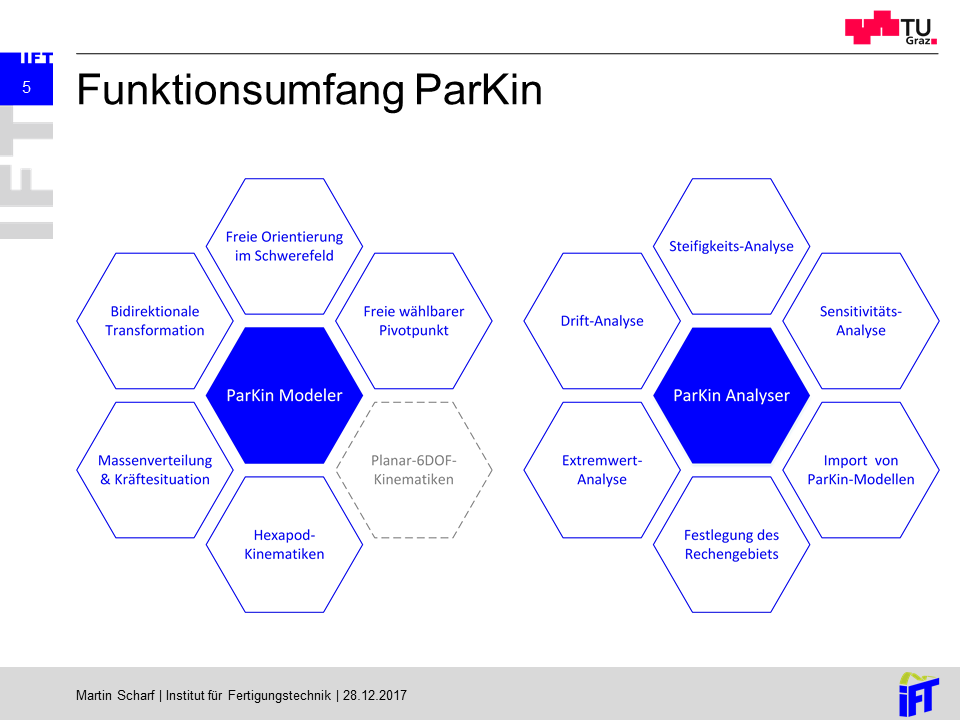
\includegraphics[width=0.7\textwidth]{method/parkin2}
    \caption[Folie]{Folie, Quelle: Eigene Darstellung}
    \label{fig:parkin2}
\end{figure}

\thispagestyle{scrheadings}
\section{Extremwert-Analyse}
\label{method-extreme}

\begin{figure}[H]
    \centering
    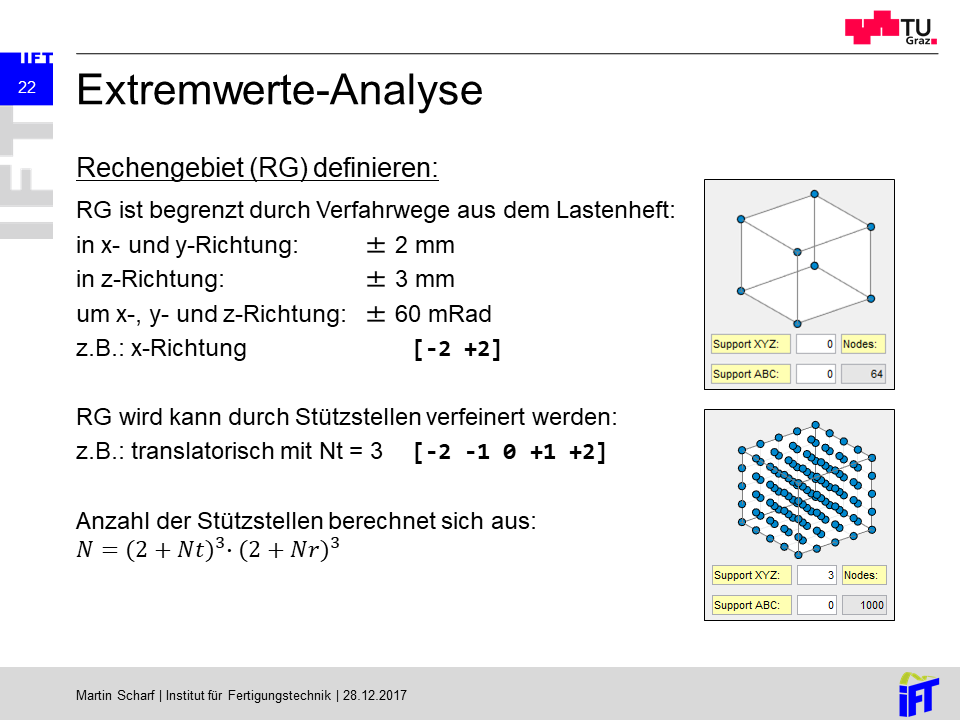
\includegraphics[width=0.7\textwidth]{method/extreme1}
    \caption[Folie]{Folie, Quelle: Eigene Darstellung}
    \label{fig:extreme1}
\end{figure}

\begin{figure}[H]
    \centering
    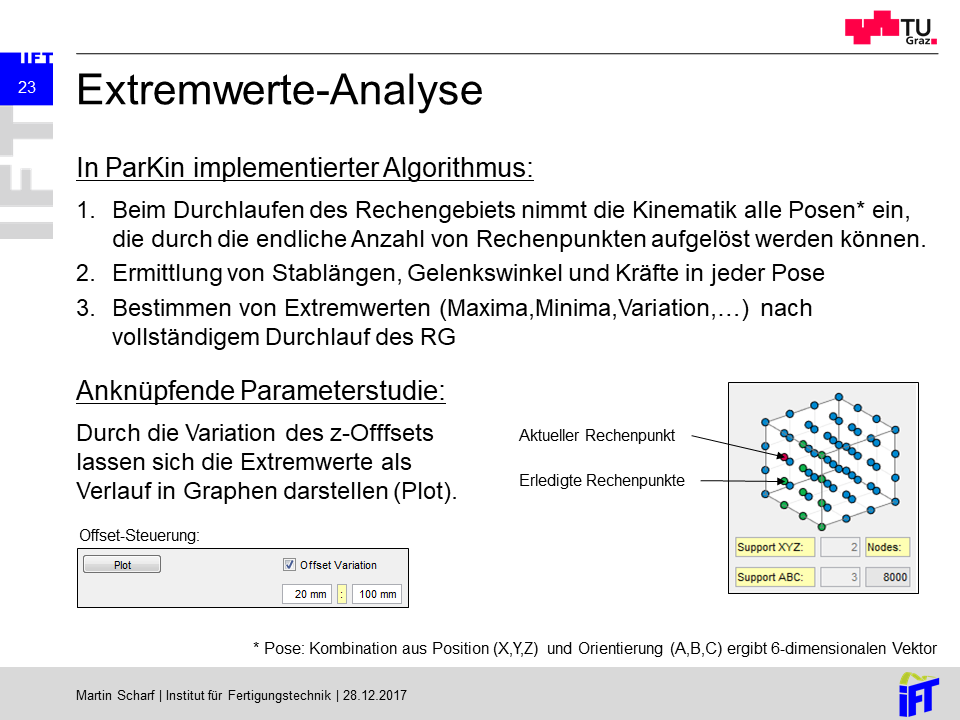
\includegraphics[width=0.7\textwidth]{method/extreme2}
    \caption[Folie]{Folie, Quelle: Eigene Darstellung}
    \label{fig:extreme2}
\end{figure}

\thispagestyle{scrheadings}
\section{Drift-Analyse}
\label{method-drift}

\begin{figure}[H]
    \centering
    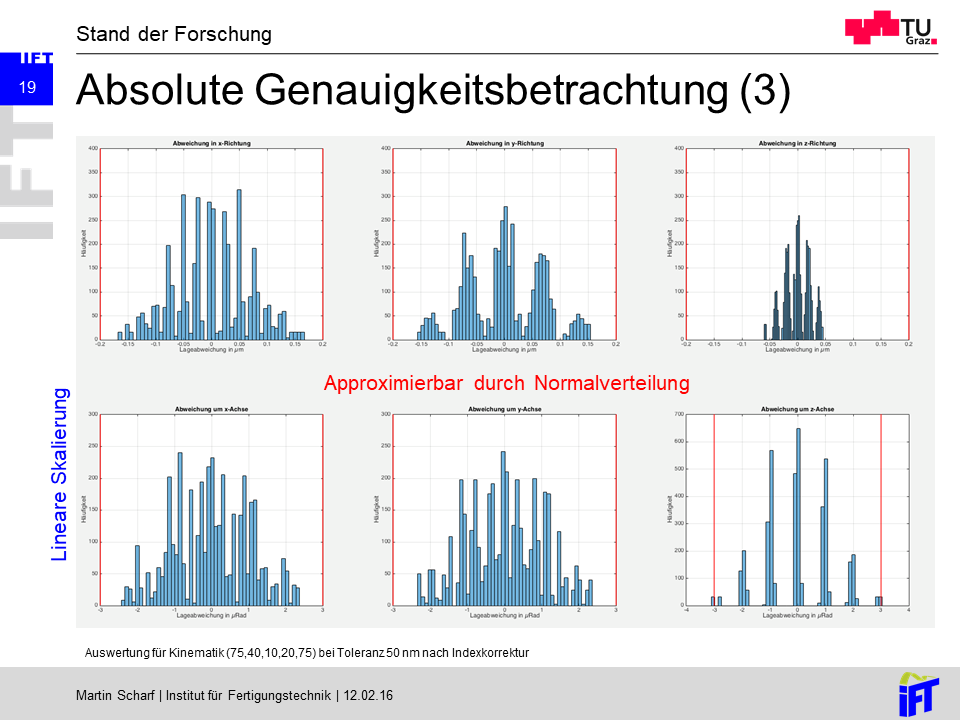
\includegraphics[width=0.7\textwidth]{method/drift1}
    \caption[Folie]{Folie, Quelle: Eigene Darstellung}
    \label{fig:drift1}
\end{figure}

\begin{figure}[H]
    \centering
    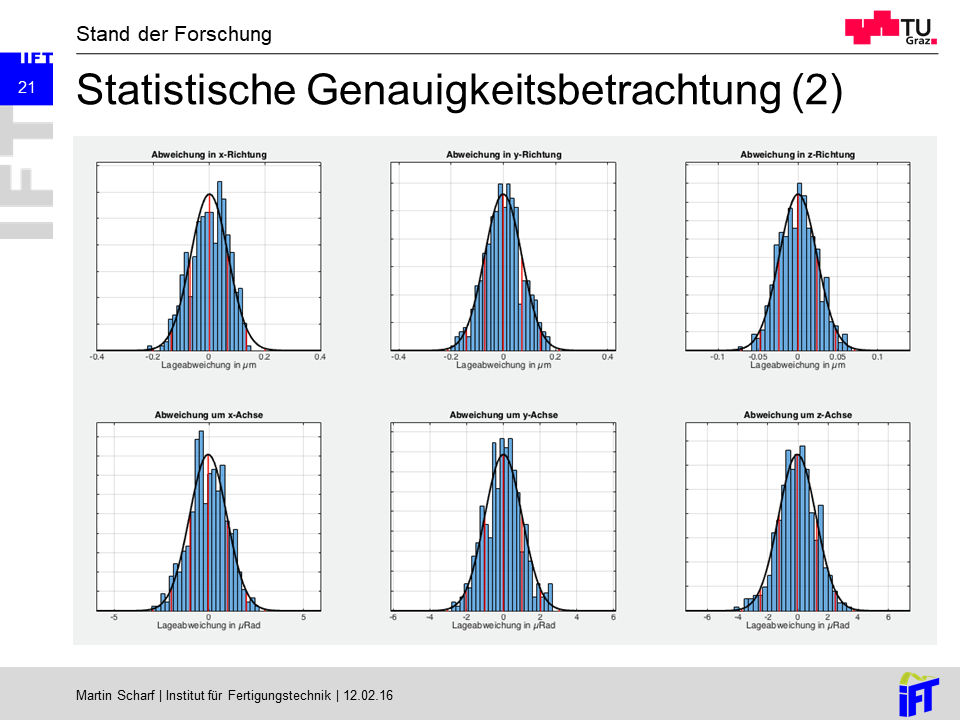
\includegraphics[width=0.7\textwidth]{method/drift2}
    \caption[Folie]{Folie, Quelle: Eigene Darstellung}
    \label{fig:drift2}
\end{figure}

\begin{figure}[H]
    \centering
    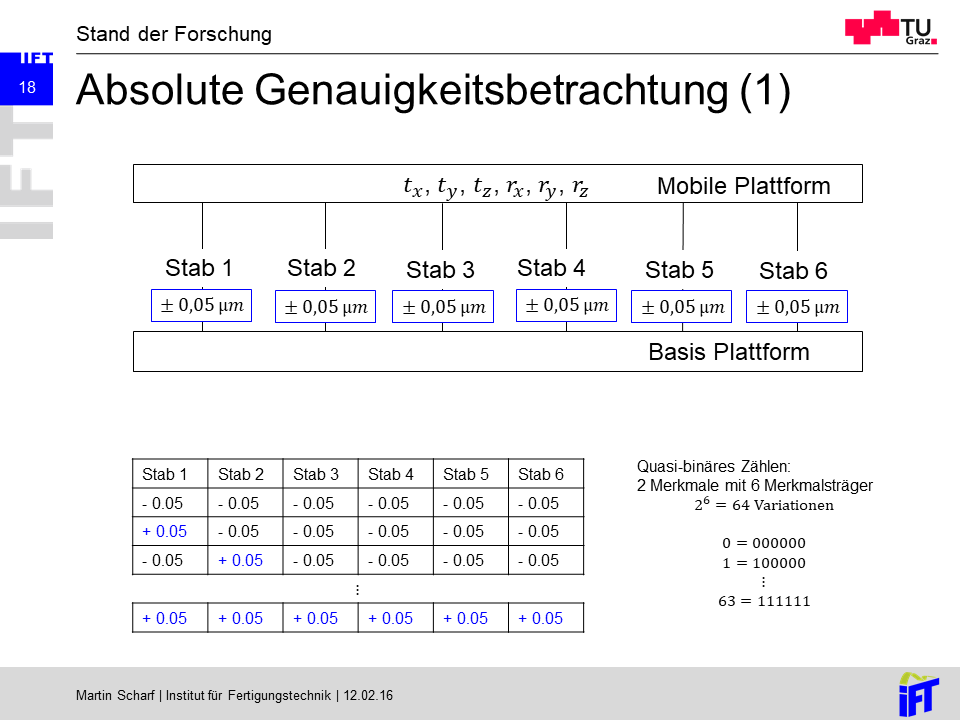
\includegraphics[width=0.7\textwidth]{method/drift3}
    \caption[Folie]{Folie, Quelle: Eigene Darstellung}
    \label{fig:drift3}
\end{figure}

\begin{figure}[H]
    \centering
    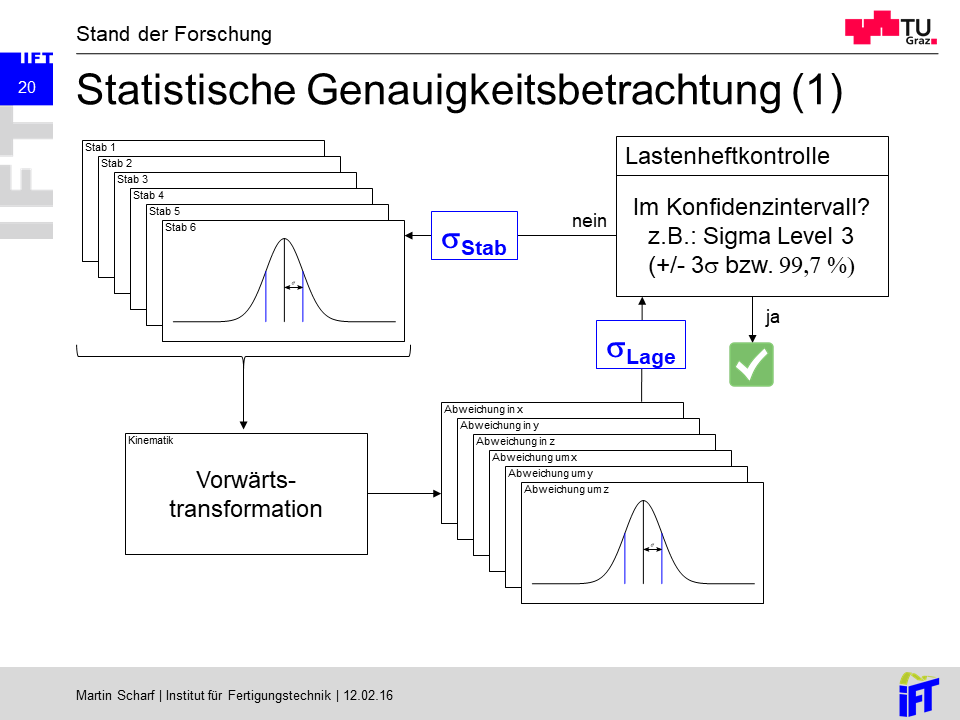
\includegraphics[width=0.7\textwidth]{method/drift4}
    \caption[Folie]{Folie, Quelle: Eigene Darstellung}
    \label{fig:drift4}
\end{figure}

\thispagestyle{scrheadings}
\section{Steifigkeits-Analyse}
\label{method-stiff}

\begin{figure}[H]
    \centering
    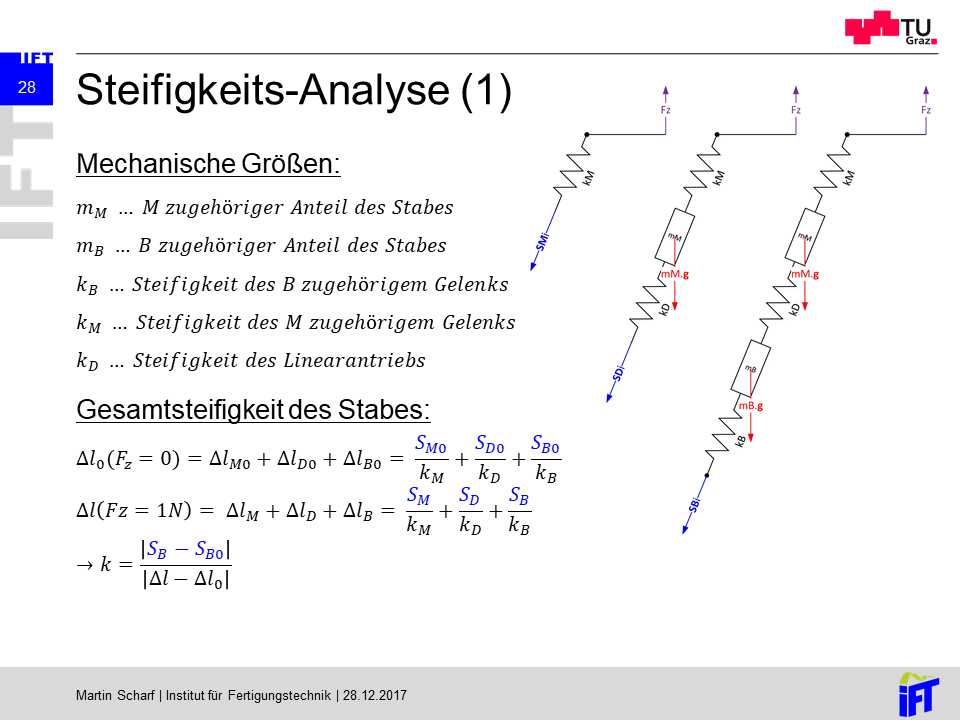
\includegraphics[width=0.7\textwidth]{method/stiff1}
    \caption[Folie]{Folie, Quelle: Eigene Darstellung}
    \label{fig:stiff1}
\end{figure}

\begin{figure}[H]
    \centering
    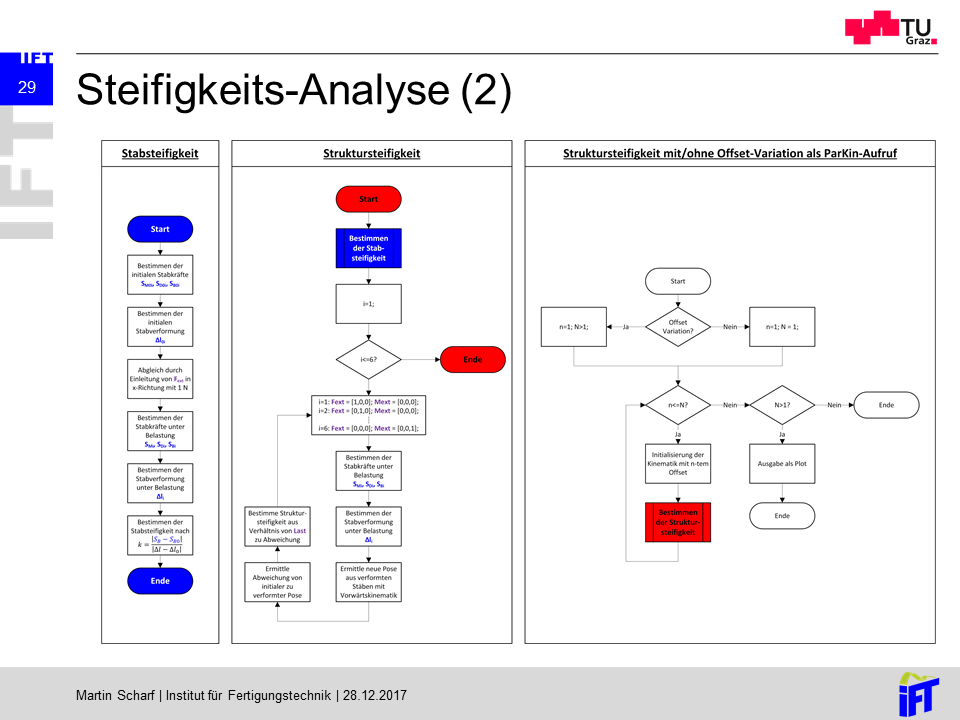
\includegraphics[width=0.7\textwidth]{method/stiff2}
    \caption[Folie]{Folie, Quelle: Eigene Darstellung}
    \label{fig:stiff2}
\end{figure}

\begin{figure}[H]
    \centering
    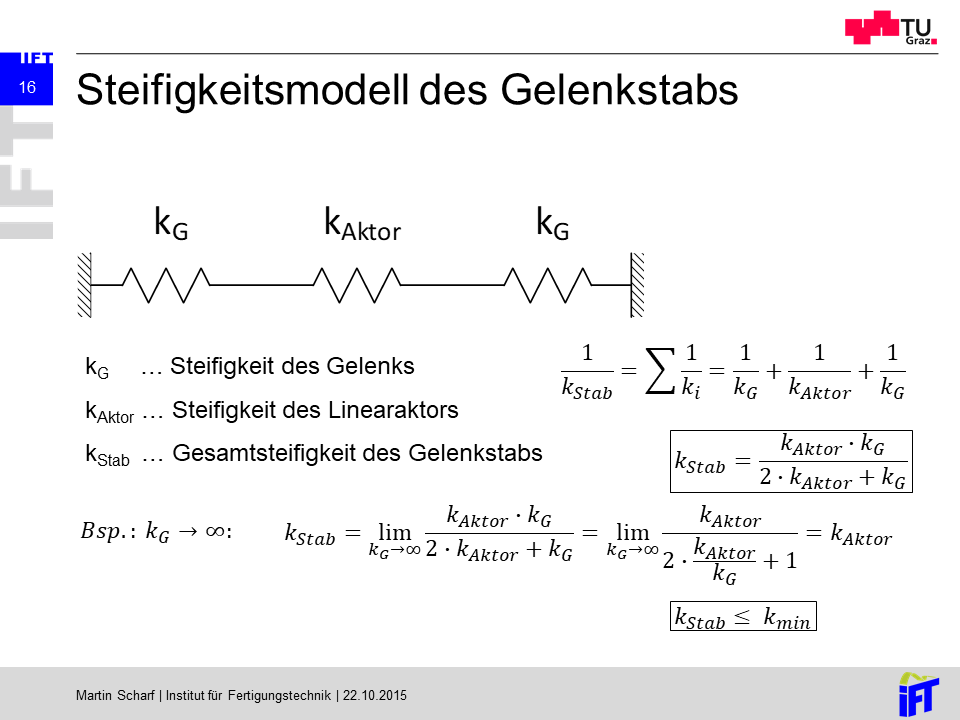
\includegraphics[width=0.7\textwidth]{method/stiff3}
    \caption[Folie]{Folie, Quelle: Eigene Darstellung}
    \label{fig:stiff3}
\end{figure}

\begin{figure}[H]
    \centering
    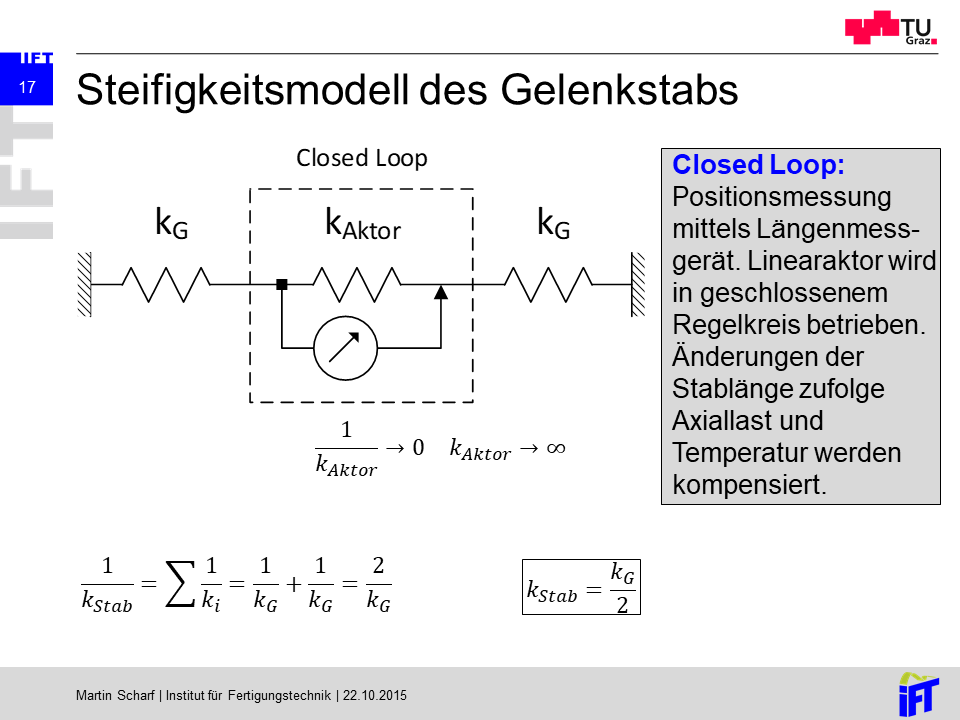
\includegraphics[width=0.7\textwidth]{method/stiff4}
    \caption[Folie]{Folie, Quelle: Eigene Darstellung}
    \label{fig:stiff4}
\end{figure}

\thispagestyle{scrheadings}
\section{Sensitivitätsanalyse-Analyse}
\label{method-sens}

\begin{figure}[H]
    \centering
    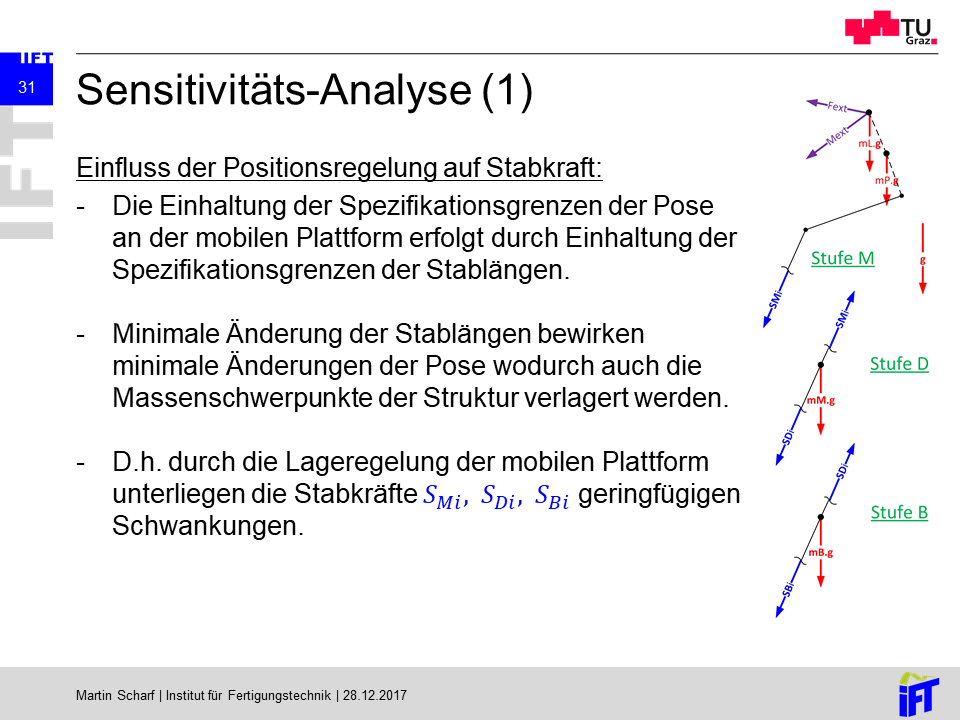
\includegraphics[width=0.7\textwidth]{method/sens1}
    \caption[Folie]{Folie, Quelle: Eigene Darstellung}
    \label{fig:sens1}
\end{figure}

\begin{figure}[H]
    \centering
    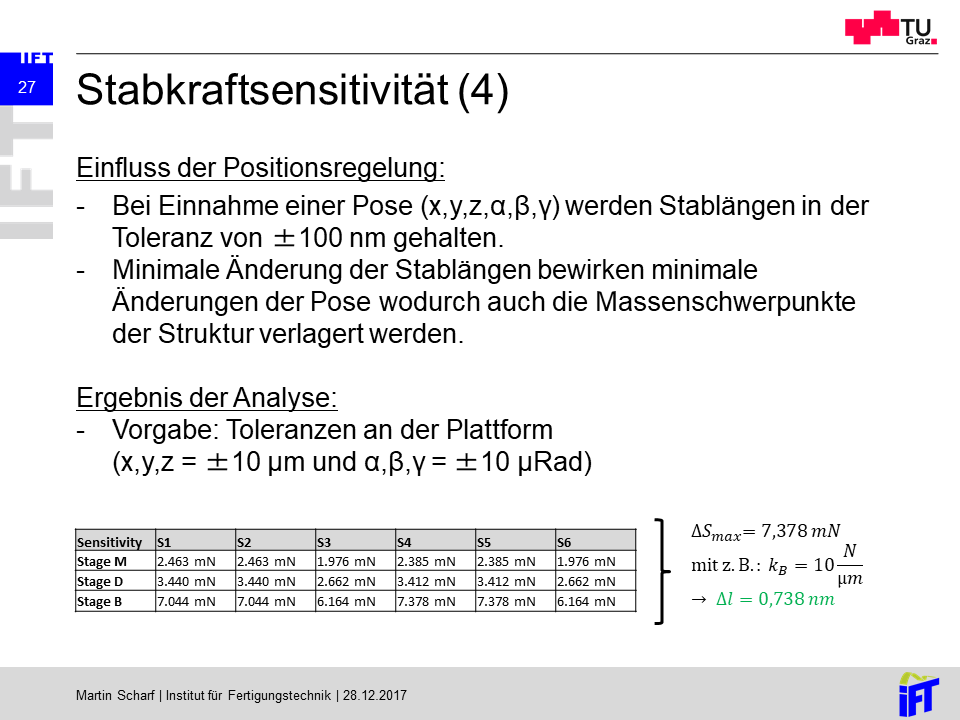
\includegraphics[width=0.7\textwidth]{method/sens2}
    \caption[Folie]{Folie, Quelle: Eigene Darstellung}
    \label{fig:sens2}
\end{figure}

\begin{figure}[H]
    \centering
    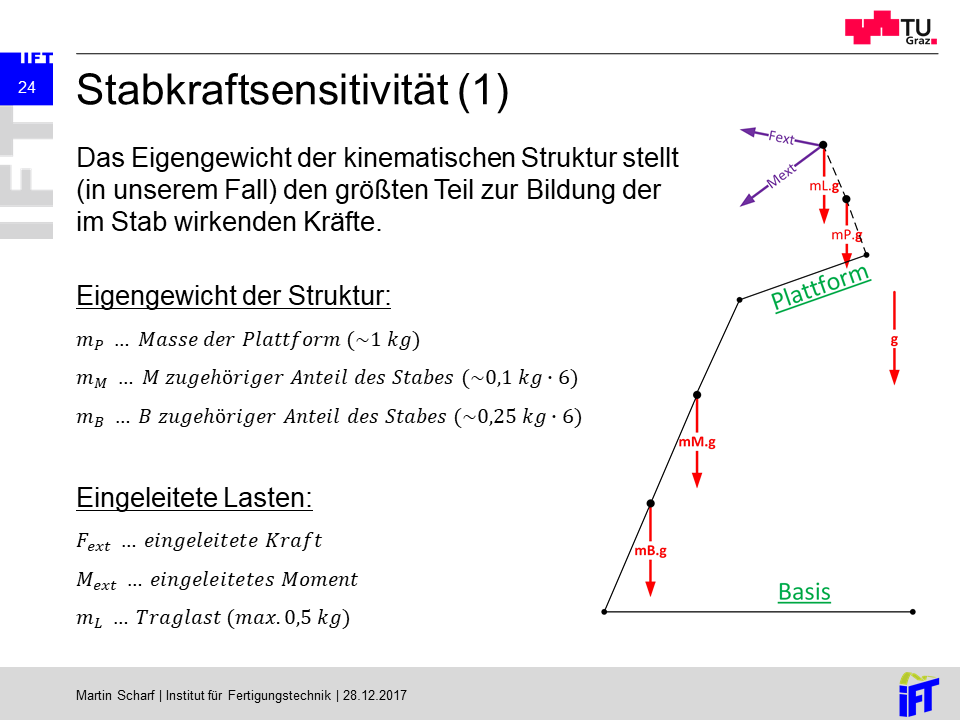
\includegraphics[width=0.7\textwidth]{method/sens3}
    \caption[Folie]{Folie, Quelle: Eigene Darstellung}
    \label{fig:sens3}
\end{figure}

\begin{figure}[H]
    \centering
    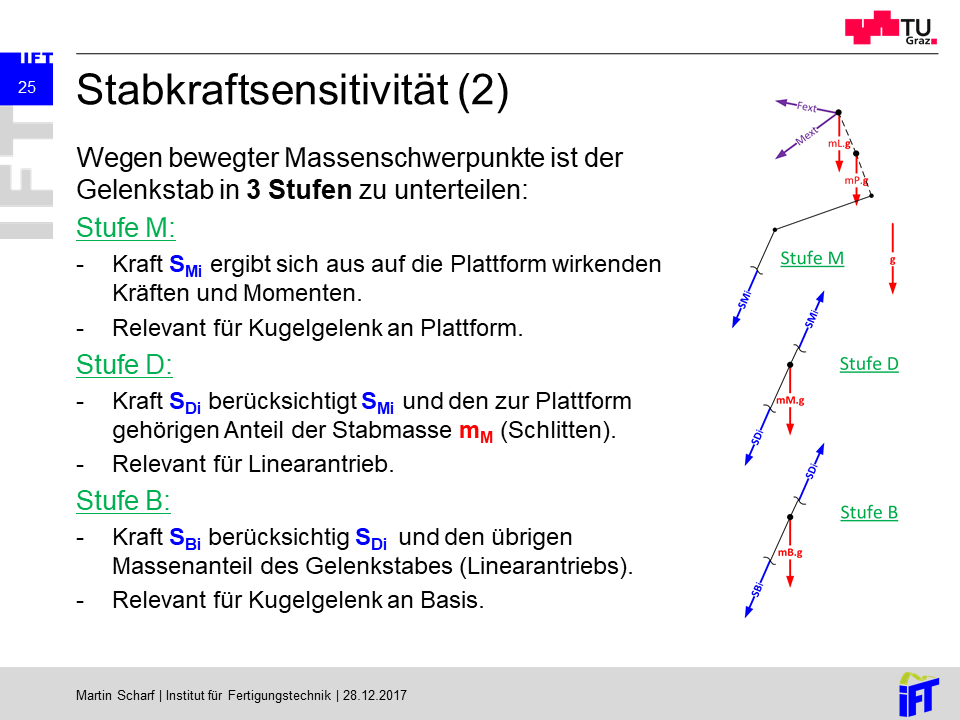
\includegraphics[width=0.7\textwidth]{method/sens4}
    \caption[Folie]{Folie, Quelle: Eigene Darstellung}
    \label{fig:sens4}
\end{figure}